%{{{ preamble
% Note: The order of some of these packages are important.
% fleqn left alligns all equations. Using settings from uiophd.cls.
\documentclass[altfont, fleqn]{uiophd}
\usepackage[T1]{fontenc}
\usepackage[utf8]{inputenc}
\usepackage[usenames,dvipsnames,svgnames]{xcolor}			
% Rebinds commands safer than using \let\mycref\cref.
\usepackage{letltxmacro}
% Can change properties of sections, such as color. 
\usepackage{titlesec}		
% Adds customizable headers and footers. 
\usepackage{fancyhdr}		
% Adds small toc lists. 
\usepackage{titletoc}		
\usepackage{hyperref}
\usepackage{graphicx}
% Essential math package.
\usepackage{amsmath}		
% \abs and \norm.
\usepackage{commath}		
% Do not know.
\usepackage{textcomp}
% SI units package.
\usepackage[redefsymbols=false]{siunitx}		
% Some extra signs and other fonts.
\usepackage{bm,upgreek} 
\usepackage{appendix}
\usepackage[
	backend=biber,
	style=numeric,
	doi=false,
	% isbn=false, 
	maxcitenames=2,
]{biblatex}
% Place figures inline with text.
\usepackage{wrapfig}
% Have to import this at the end for this to work somehow.
\usepackage{cleveref}		
\usepackage{multicol}
% Caption options. Used to change label color.
\usepackage{caption}
% Commands that help placing figures side by side.
\usepackage{subcaption}
% Used with minted to get caption on top.
\usepackage{floatrow}
% Highlighting of source code.
\usepackage{mdframed}
\usepackage{minted}
\usemintedstyle{manni}
\floatsetup[listing]{style=Plaintop}
% \surroundwithmdframed{minted}
% \BeforeBeginEnvironment{minted}{\begin{mdframed}}
% \AfterEndEnvironment{minted}{\end{mdframed}}
    

% Glossary packages.
% \usepackage[nopostdot,toc]{glossaries}
% % Enables multi column glossary.
% \usepackage{glossary-mcols}
% % Necessary for the glossaries package.
% \makeglossaries

\addbibresource{master.bib}

% Remove certain fields from appearing in the bibliography.
\AtEveryBibitem{\clearfield{month}}
\AtEveryBibitem{\clearfield{day}}
\AtEveryBibitem{\clearfield{note}}
\AtEveryCitekey{\clearfield{month}}
\AtEveryBibitem{%
    \ifentrytype{misc}
    {%
    }%
    {%
        \clearfield{url}
        \clearfield{urldate}
    }%
}

% Use ampersand "&" instead of "and". 
\renewcommand*{\finalnamedelim}{%
    \ifnumgreater{\value{liststop}}{2}{\finalandcomma}{}%
    \addspace\&\space%
}
% Paper properties. 
\pagestyle{fancy}
% Removes the header bar and text.
\renewcommand{\headrulewidth}{0pt}
\fancyhead{}
% Custom colors.
\definecolor{viridis_01}{rgb}{0.267004, 0.048740, 0.329415}
\definecolor{viridis_02}{rgb}{0.190631, 0.407061, 0.556089}
\definecolor{viridis_03}{rgb}{0.208030, 0.718701, 0.472873}
\definecolor{viridis_04}{rgb}{0.993248, 0.906157, 0.143936}
% Change section formatting.
\titleformat{\section}
    {\color{viridis_02}\Large\bfseries}
    {\color{viridis_02}\thesection}{1em}{} 		
% Change section formatting.
\titleformat{\subsection}
    {\color{viridis_02}\large\bfseries}	
    {\color{viridis_02}\thesubsection}{1em}{}
% Change section formatting.
\titleformat{\chapter}[hang] 				
    {\bfseries\Huge} 	
    {\color{viridis_01}\thechapter\hspace{20pt}\rule[-3pt]{2pt}{23pt}\hspace{10pt}}
    {0.5ex} 			
    {\color{viridis_01}} 	
    [
        % This will be applied after each chapter?
        %\small
        %\startcontents
        %\printcontents{}{1}{\setcounter{tocdepth}{1}}
    ]		
% Change the color of every citation.
\AtEveryCite{\color{viridis_03}}
% Hyperlink colors. 
% Empty color disables coloring.
\hypersetup{
	colorlinks=true,
	citecolor=viridis_03,
	filecolor=black,
	linkcolor={},
	urlcolor=black,
}
% Change the color of caption labels.
\captionsetup{labelfont={color=viridis_03}}

% Glossary settings commented out:
% % Change the color of the glossary commands \gls and \Gls.
% \LetLtxMacro{\mygls}{\gls}
% \renewcommand{\gls}[1]{{\color{viridis_03}\mygls{#1}} }
% \LetLtxMacro{\myGls}{\Gls}
% \renewcommand{\Gls}[1]{{\color{viridis_03}\myGls{#1}} }
% % Include the glossary file. 
% \newglossaryentry{regspike}{
    name={regular spiking},
    description={Often compared to fast spiking}
}

\newglossaryentry{fastspike}{
    name={fast spiking},
    description={A short durtion extracelluar spike}
}


% % Change the emph command.
% \DeclareTextFontCommand{\emph}{\color{viridis_03}}
% Change color of clever ref.
\AtBeginDocument{
    \LetLtxMacro{\mycref}{\cref}
	\renewcommand{\cref}[1]{{\color{viridis_03}\mycref{#1}}}
    \LetLtxMacro{\myCref}{\Cref}
	\renewcommand{\Cref}[1]{{\color{viridis_03}\myCref{#1}}}
    \LetLtxMacro{\mynameref}{\nameref}
	\renewcommand{\nameref}[1]{{\color{viridis_03}\mynameref{#1}}}
    % \LetLtxMacro{\myfullref}{\fullref}
	% \renewcommand{\fullref}[1]{{\color{viridis_03}\myfullref{#1}}}
}
% % Change the spacing of some math symbols in math mode.
% \setlength{\thickmuskip}{6pt}
%}}} end of preamble
\begin{document}
%{{{ Abstract
\chapter*{Abstract}
\noindent
The physical processes that creates electrical signals in neurons are well understood, 
but how the signals are processed into actions and thoughts has yet to 
receive a scientifically robust answer
Cell type classification is of high importance because the function of different 
neurons is still largely a mystery. 
%}}} end of Abstract
%{{{ Table of Contents
\setcounter{tocdepth}{1}
\startcontents
\tableofcontents
%}}} end of Table of Contents
%{{{ Introduction
\chapter{Introduction}

% Since 
% the conception of neuroscience the neurons function have been studied on many levels
% from the properties of the cell membrane to clustered networks of neurons.

% TODO: COPY Vigneswaran.
Early investigators first suggested that
interneurons, with high spontaneous firing rates, had “thin” ac-
tion potentials of short duration and could be distinguished from
pyramidal cells with longer action potentials and lower, regular
spiking pattern of discharge (Mountcastle et al., 1969). These
differences were subsequently confirmed by detailed intracellular
studies in brain slices from rodents (Connors et al., 1982; McCor-
mick et al., 1985; Contreras, 2004).

There are several types of neurons 
and it was early noticed that the discharge waveform
had different shapes
for different types on neurons.
%TODO: Source

The behaviour of neuronal circuits is heavily effected by the kinds of neurons
it has. 
Investigating the different kinds of is therefor of major importance. 
The majority of studies that use  extracellular recordings ignore 
neuronal types, while some studies have attempted to classify
neurons based on signal waveforms and spike patterns. 
% TODO: SOURCE

% TODO: COPY katai
Intracellular recordings in slice
preparations have demonstrated that c-aminobutyric acid (GABA)-
containing, inhibitory interneurons produce action potentials of a
much shorter duration than excitatory, pyramidal neurons (McCormick
et al., 1985).

% TODO: COPY katai
Based on this finding, some extracellular recording
studies distinguished neuronal types based mainly on the differences
in spike width (Wilson et al., 1994; Constantinidis \& Goldman-Rakic,
2002; Mitchell et al., 2007; Cohen et al., 2009).
However, the identification of neuronal types by their spike width
alone has several problems. First, in extracellular recording conditions,
the measurement of spike width is often disturbed by background
noise near the baseline and the filtering parameters used in the
experiment. Second, it has become clear that not all short-duration
action potentials are generated by fast spiking (FS) interneurons.
Intracellular studies have documented short-duration action potentials
in a number of neurons that were subsequently labeled and shown to
have a pyramidal morphology (Nowak et al., 2003).

In addition measurements from some pyramidal axons has been shown
to give shorter duration action potentials (Robbins 2013).
%(Vigneswaran 2011).

% TODO: COPY Bartho 2004
In the hippocampus, the combination of several extracellular
features, such as spike duration, firing rate, and pattern and
spike waveform, reliably separates pyramidal cells from inter-
neurons (Csicsvari et al. 1999). The validity of neuron classi-
fication on the basis of extracellular features has been sup-
ported by in vivo intra- and juxtacellular labeling as well as
simultaneous extra- and intracellular recordings from the same
neurons (Henze et al. 2000; Klausberger et al. 2003; Sik et al.
1995). Similar classification criteria are not available in the
neocortex. Mountcastle et al. (1969) have noted that the occa-
sionally recorded “thin spikes” in the somatosensory cortex
had different response properties than the majority of units and
suspected that they were interneurons. Other observations in-
dicated that fast-spiking neurons have receptive and evoked
response properties different from the majority of slower, more
regular firing cells (Constantinidis and Goldman-Rakic 2002;
Simons 1978; Swadlow 2003; Swadlow and Gusev 2002;
Swadlow and Lukatela 1996; Swadlow et al. 1998). Intracel-
lular recordings and labeling in cortical slices showed numer-
ous classes of interneurons on the basis of the firing rates, spike
morphology, and spike dynamics (Connors et al. 1982; Gupta
et al. 2000; Kawaguchi and Kubota 1993; Somogyi et al.
1998). However, the information gathered in intracellular ex-
periments in vitro cannot be directly applied to extracellularly
recorded spikes in the intact brain. Furthermore, intra- and
juxtacellular studies carried out in vivo do not directly support
the suggestion that fast firing neurons unequivocally identify
interneurons (Azouz et al. 1997; Degenetais et al. 2002; Doug-
las et al. 1995; Gray and McCormick 1996; Steriade et al.
1998).

Another popular approach is classifying based on discharge patterns, 
such as bursting behaviour and inter spike interval (ISI).
Classification based on inter spike bursting behavior and ISI has
gained more traction than soley using spike waveform. 
% Though classification based on discharge pattern has been accepted
% as a better method than using the waveform, 

These classifications are often based
on the response of a current pulse which makes them difficult
to apply on recordings from
in vivo measurements. 
% Taking another approach, recent intracellular recording studies have
% revealed that cortical neurons can be classified into four types by their
% discharge patterns in response to current pulses 
(Kang \& Kayano,
1994; Gray \& McCormick, 1996; Nowak et al., 2003; González-
Burgos et al., 2004, 2005a,b).

% The problem
% While doing single cell recordings the only information
% about the neuron that is avaiable is the electric signal from the neuron.
Modern types of 
classification uses genotype?, the structure of the neuron and the 
electric signal.

While doing single cell recordings on alive subjects the researchers are
recording in the dark. 

In this article we show that interneurons can be seperated from pyramidal
neurons based on data and models from the Blue Brain project. 
The program makes an easy way to do the same analysis
on future models as long as the models can be loaded with LFPy.


%}}} end of Introduction
%{{{ Theory
\chapter{Theory}
% NOTE: 
% The physical processes in and around neurons are well understood in comparison
% to the function they serve. 
% The basic function of a neuron is to receive and send 
% action potentials, 
% but what exact information is being transmitted or how 
% it is processed into thoughts does still not have a conclusive answer.

\vspace{1em} 
\startcontents
\printcontents{}{1}{\setcounter{tocdepth}{2}}
  
%{{{ The Neuron
\section{The Neuron}
\begin{figure}[h]
    \centering
    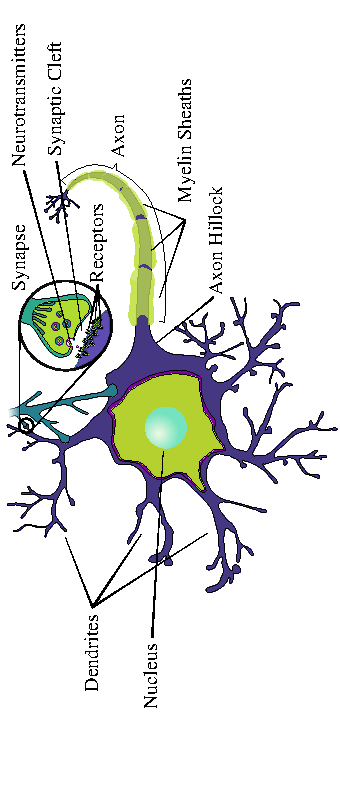
\includegraphics[angle=-90,width=1.0\textwidth]{images/2_1/neuron_structure.pdf}
    \caption{}
    \label{fig:2_1_neuron}
\end{figure}
\noindent
{Neurons} 
are electrically excitiable cells
that are a fundamental part of all brain functions.
Other names include {nerve cells}, {neurone} or more 
colloquially {brain cells}.
Neurons form in big networks 
which process information,
and in the human brain there is an estimated $10^{11}$ neurons.

Special proteins in the cell membrane enables the neuron to
fire action potentials when it is electrically excited. 
These action potentials are sharp voltage changes that propagates through
the full structure of the neuron.
The same properties that makes the neuron able to fire makes 
the action potential {regenerative}, meaning it will propagate
without decay.

The body of the neuron, the {soma}, has {dendrites} and 
the {axon} attached to it. 
The dendrites and the axon are very thin branching structures 
with a width usually in the order of \SI{1}{\micro\metre}. 
While neurons often have many dendrites directly attached to the soma
there is only one axon attached to the soma at the axon hillock.
The axon can branch several times before it ends and 
usually connects to the dendrites of other neurons via synapes.

The synapes are electrically sensitive which allows information
to pass between neurons. 
Though the majority of all synapes are axo-dendritic 
(axon to dendrite),
other junctions are also possible.
Other junctions include but are not limited to,
dendrite to dendrite, 
axon to axon and 
axon to blood vessel. 
When an action potential reaches a synapse it will activate
the synapse and pass information to the connect neuron. 
The information that is passed along depends on the type of synapse,
and if it is of a chemical or electrical type.

% NOTE: Topic to mention:
% Neuron cell types, pyramidal neurons, basket neurons interneurons, what 
% are they. The term "morphology". Intracellular also referred to as membrane potential.
% Subcortical. Se hemalainen p.421. for a good summary. What is transmembrane current. 
% Impulse. Apical dendrites. Grey matter. Spines. Synapses. Quiescent neuron.

%}}} end of The Neuron
%{{{ Electrical Activity
\section{The Cell Membrane}
\begin{figure}[h]
    \centering
    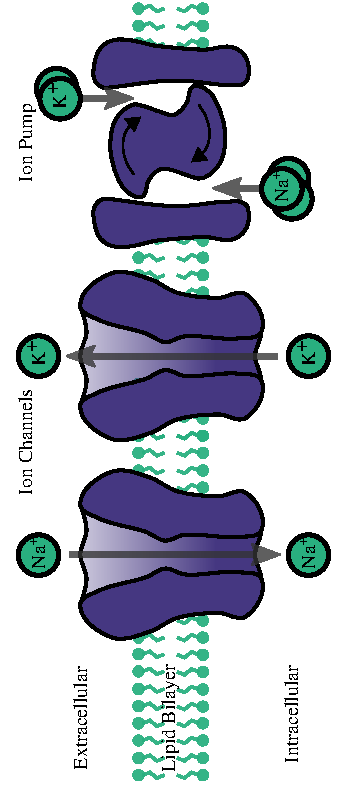
\includegraphics[angle=-90,width=1.0\textwidth]{images/2_1/ion_pumps_0.pdf}
    \caption{
        Common portrayal of ion channels and pumps in the neuron cell membrane. They are responsible for
        creating a potential gradient across the membrane. 
        Ion channels have
        selective permeability of ions. Ion pumps activly transport ions
        through the membrane, often against the potential gradient. 
        Image modified from 
        \textcites{sterratt_principles_2011}.
    }
    \label{fig:2_ion_channels}
\end{figure}
The potential difference between the inside and outside the neurons 
are caused by different concentrations of 
ions
in the extracellular and intracellular medium. 
The ions cannot pass through 
the cell membrane as it
consists of a \SI{5}{\nano\metre} lipid bilayer which is mostly impenetrable 
to ions. 

In the membrane sits ion channels and 
ion pumps which can have selective permeability to ions. 
Collectivly they are refered to as ion transporters. 
These are created by proteins in complicated shapes. 
There and there are over 200 
kinds of electrically sensitive ion channels.
Together they create a 
potential gradient across the membrane. 
The most significant ions in this process are Sodium (Na$^+$), Potassium (K$^+$), 
Calcium (Ca$^{2+}$), Magnecium (Mg$^{2+}$) and Chloride (Cl$^{-}$). 
Ion channels are divided between passive channels and 
active channels where the active channels can change 
permeability under certain conditions while passive channels have a constant
permeability. 
\Cref{fig:2_ion_channels} shows a common portrayal of ion channels and pumps. 

The ion pumps differ from the channels by activly transporting certain
ions through the membrane. 
For instance, the Sodium-Pottasium exchanger pushes two K$^+$ ions out of the cell
for every three Na$^+$ it pushes into the cell. Doing this creates a net 
loss of charge inside the cell and the pump is therefore electrogenic. 
Not all pumps are electrogenic, the Sodium-Hydrogen exchanger transports
H$^+$ and Na$^+$ without effecting the net charge.
For each H$^+$ ion out of the cell the pump pushes one Na$^+$
into the cell. 

To understand the electrical activity of neurons it is useful
to view the neuron as an electronic circuit where the ion channels, ion pumps
and the membrane serve as different electronic components.
\Cref{fig:2_hud_hux} shows the electronic circuit used by hudgkin
and huxley in their original description of a neuron membrane. 
% Here the ion pump has been ignored as the concentrations were 
% assumed to be constant at boths sides of the membrane in their model.

\begin{figure}[h]
    \centering
    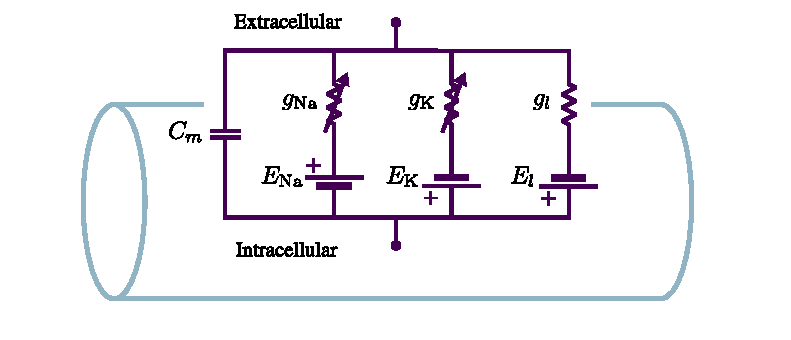
\includegraphics[width=1.0\textwidth]{images/2_1/compartment.pdf}
    \caption{Them compartment.}
    \label{fig:2_hud_hux}
\end{figure}

\textcites{hodgkin_quantitative_1952,connor_prediction_1971,sterratt_principles_2011}
% The temperature is important.
%}}} end of Neuronal Models
%{{{ Ciruit Model 
\section{Circuit Model}
Hudgking and Huxley originally tried to understand the
electrical properties of neuron by studing squid axons. 
Given very spesific functions for the active conductances $g_\text{Na}$
and $g_\text{K}$, this circuit is enough to describe an important feature
of neurons, called action potentials.
The model was developed by recording the activity of each
type channel in the membrane. 
The model of each channel was then constructed by fitting 
the data to functions. 
The final model of the cell membane was then constructed 
by incorperating each channel model. 

%}}} 
%{{{ Action Potential
\section{Action Potential}
Action potentials are sharp increases in the membrane potential
followed by a less sharp decrease towards the resting potential. 
In the the depolarization phase the potential rises towards the peak magnitude, 
while in the repolarization phase the potential decreases towards
the cells resting potential.
When the potental is below the resting potential 
it reaches the afterhyperpolarization phase before
it returns to its resting potential.

%}}} end of Action Potential
% Neuron Models {{{ %
\section{Compartmental Models}
There are multiple models for neurons, some of the main groups are 
point models and compartmental models. List many models?
Multi-compartmental models 
can be useful to understand the processing of neurons with
complex morphological structures
\begin{figure}[h]
    \centering
    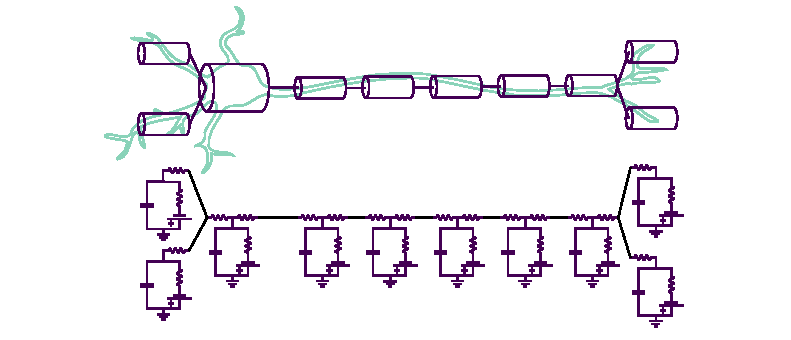
\includegraphics[width=1.0\textwidth]{images/2_1/compartments.pdf}
    \caption{Compartmental model.}
    \label{fig:2_comp_mod}
\end{figure}
% }}} 
%{{{ Electrodes
\section{Electrodes}

%}}} end of Electrodes
%{{{ Extracellular
\section{Calculating Extracellular Potential}
The extracellular potential is the electric potential generated from the transmembrane
currents in the neurons. When a neuron fires this can be seen from the extracellular
potential which will have a spike which is similar to the intracellular spike.

By modelling the neuron as
compartments and approximating each compartment as
a spherical volume current source at position $\bf r_0$, the potential at 
at position $\bf r$ at time $t$ will be,
\begin{align}
    {\bf E(r, t)} = \frac{1}{4\pi\sigma}\frac{I_0(t)}{\abs{\bf r - r_0}}
\end{align}

\begin{align}
    {\bf E(r, t)} = \sum^N_{n=1} \frac{1}{4\pi\sigma}\frac{I_n(t)}{\abs{\bf r - r_0}}
\end{align}

Potential from compartments modelled as line sources. 
\begin{align}
    {\bf E(r, t)} &= \frac{1}{4\pi\sigma}\sum^N_{n=1}I_n(t)\frac{dr_n}{\abs{\bf r - r_0}}\\
    &= \frac{1}{4\pi\sigma}\sum^N_{n=1}I_n(t)
        \frac{1}{\Delta s_n}
        \log\abs{\frac{\sqrt{h_n^2 + \rho_n^2} - h_n}{\sqrt{l_n^2 + \rho_n^2} - l_n}}
\end{align}
Taken from \textcite{linden_lfpy:_2013}


This equation rests on two assumptions,
\begin{enumerate}
	\item The permeability $\mu $ of 
	the extracellular medium is the same as that of vacuum $\mu_0$.
	\item The quasistatic approximation which lets the 
	time derivatives, $\partial E/\partial t$, 
	be ignored as source terms.  See \cref{sec:quasi}
\end{enumerate}

The extracellular potential can be calculated
using Maxwell's equations and the continuity equation if the spatial
distribution (morphology) of transmembrane currents and the extracellular conductivity
is known. 



In the quasistatic approximation, since $\nabla\times\bf E = 0$, the
electric field can be expressed with a scalar potential.

Forward problem = calculate the potential from the current source, inverse problem is used
in magnetoenchephalography (important).
The amplitude of a spike in the
extracellular potential is usually in the magnintude of
$< 200 \upmu$V.  
The noise of electrodes vary, but can be as much as $20 \upmu$V. 
This limits the range electrodes can record from. 

The currents sum to zero, while the spike is very visible, there are many small currents
in the dendrites with opposite current. 
(\cite{hamalainen_magnetoencephalography-_1993})

The extracellular spike width tend to increase with distance from soma because of the
neuronal morphology. 
This article used a passive neuron model with different morphologies to show
that the spike width increases with distance to soma. The spike amplitude also
decreases with distance to soma and seems to follow a power law. 
(\cite{pettersen_amplitude_2008} \hspace{-3pt}).

The shape of extracellular spikes are mainly depedent on the membrane currents
and the morphology of the cell. 
Some of the effects from the morphology of the cell are increased spike width and
decreased amplitude from distance to soma. 

Many things here from around page 245. 
When the conductivity $\sigma$ and the current generators are know, Maxwell's
equations and the continuity equation equation can be used to calculate the electric
field $E$ and magnetic field $B$. (TODO: Copied text)
(\cite{hamalainen_magnetoencephalography-_1993})

\subsection*{Background}
% Electric potential from neurons can either be obtained 
% by measuring the membrane potential or measured from the extracellular
% medium. 
%Recording the membrane potential is easier to interpret but harder to execute 
%while 
%extracellular recordings are harder to interpret but easier to execute. 
Recording is usually done using electrodes, this makes recording the membrane potential
more challenging than recording from the extracellular medium as the electrode
has to be very close or inside the cell. 
At the time of writing,
recording the membrane potential of a concious subject is nearly impossible,
this makes understanding extracellular potentials vital for current research. 


Early calculations was done by Rall 1962 investigating 
the interaction between action potentials and synapes using cylinders
as the current source. (TODO: Read article, make more understandble.)
Holt and Koch 1999 added comparmental models to reconstruct pyramidal neurons. 

The information about the transmembrane current is usually difficult to obtain,
as well as the morphology.


%}}} end of Extracellular
%{{{ Neuron and lfpy
\section{Neuron \& LFPy }
LFPy is a Python module that uses Neuron and the mentioned methods to calculate the 
electric field outside the neuron. 
\cite{linden_lfpy:_2013}
\subsection*{Background}

%}}} end of Neuron and lfpy
%{{{ Cell classification

\section{Cell Type Classification}
It was early observed that the shape of action potentials are different for 
individual neurons. \textcite{mountcastle_cortical_1969} discovered what
they called regular spiking and fast spiking.

\cite{mountcastle_cortical_1969}.
Results are based on spike width and amplitude.
The basis for all spike shapes are the types and concentrations of
ion channels.
This is the central factor that decides if the neuron has short or long action potentials.
A number things has been observed that can change spike spike width.
Factors that change action potentials width:
* Firing frequency.
* Input current. Higher current gives higher frequency.
* Number of previous spikes.
* Bursting behavior.
* Backproagating action potentials.

% }}} end of Cell classification
%}}} end of Theory
%{{{ Methods
\chapter{Methods}
Methods mentioned here have been developed spesifically for this research. 
\vspace{1em} 
\startcontents
\printcontents{}{1}{\setcounter{tocdepth}{3}}
% Spike Width Measurement {{{ %
\section{Spike Width Measurement}
Most extracellular spikeshapes has a minimum value greater than the maximum 
value,
but this is not always the case when measuring
far away from soma. 
\\

\noindent 
{\bf Peak-to-peak Width:} Refered to as type I spike width in the code. 
The width is measured as the time from the minimum potential to the maximum. 
This is a rough measure of the time from the polarization phase to 
the afterhyperpolarization phase. 

The definition can be implemented by measuring the width from
minimum to maximum value, but in cases where the spike is flipped
the definition must also change. 
As such the implementation was done by defining the positive axis along 
the maximum absolute value and calculate the time from 
the maximum value to the preceding minimum value.
\newline

\noindent
Width Type II - Width at Half Amplitude:

Width is measured as the duration the spike is below half amplitude of the signal measured
from the baseline at the start of the signal. 
\newline

\noindent
Width Type II - Width at Half Amplitude:

Width is measured as the duration the spike is below half amplitude of the signal measured
from the baseline at the start of the signal. 
\newline


%}}} end of 
% Spike Amp. Measurement {{{ %
\section{Spike Amplitude Measurement}
Amplitude is easier to calculate than the width of a spike, 
but there are still different ways to define the amplitude. 
In most cases the amplitude is defined as the distance from a baseline,
in a similar manner as a sinusoid.
The baseline is not always well define with spikeshapes.
For the intracellular potential the baseline can for instance be set
at the firing threshold, but for extracellular spikes this is not possible.
Maybe more common is to set
the baseline as the value during quiescence. 
For modelling purposes this is can provide difficulties.

% }}} Spike Amp. Measurement %
\section{Similarity Measure}
\begin{figure}[h]
    \begin{center}
        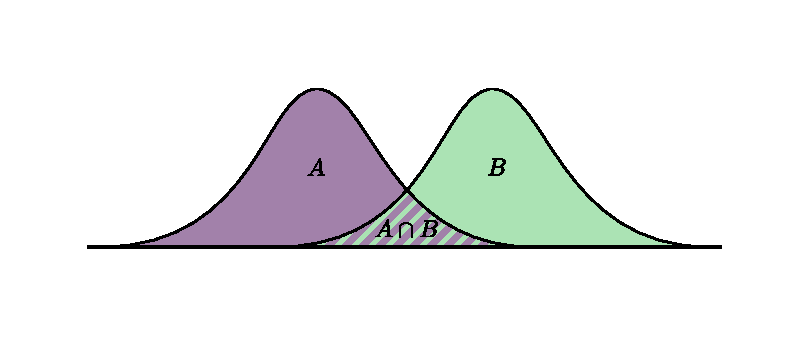
\includegraphics[width=1\textwidth]{images/sec_3/hist_inter.pdf}
        \caption{
            Nothing.
        }
        \label{fig:3_hist_inter}
    \end{center}
\end{figure}
% LFPyUtil{{{ 
\section{LFPyUtil}
% Content {{{ %
\subsection{About}
LFPyUtil is a python package that was created for this project with the purpose
to simplify the simulation pipeline for multiple neurons and creating
an easy to use interface when developing new simulations. 
LFPyUtil extends and uses the package LFPy to accomplish this. 
Simulations can be run in parallel and data from simulations can
automatically be saved and loaded to avoid unnecessary processing time.
% Some features of LFPyUtil are running simulations in parallel,
% and automatic saving and loading run parameters and data from simulations.

% TODO: Add text about NEURON, maybe skip the next paragraph.
% TODO: Link to where the programming package is saved, pypi, 
% and that it uses python 2 because of NEURON.

% TODO: This paragraph must be made clearer.
LFPy is a Python package created to calculate extracellular potentials.
Another major feature is wrapping the cell model and electrodes
from the NEURON simulation environment into Python objects, such as the 
\verb+LFPy.Cell+ and 
\verb+LFPy.StimIntElectrode+ classes.
This makes working with NEURON more pythonic as 
it can be argued that NEURON is
state-based.
That is, even though the Python interface of NEURON uses objects,
the objects are bound to the state system. 
In practical terms this means that all functions and variables
with NEURON are global static. 

While NEURON has support for paralell processing of single simulations
it does not have 
any inherit support for running multiple independent simulations.
For "embarrasingly parallel" situations like this,
users have had to resort to creating their own methods
to start each simulation independently.
For instance, one solution would be to use a Python script to run other scripts
through the command line, effectivly starting new processes.
In addition there is no function to reset the simulation environment
which can make previous simulations affect later ones.

LFPyUtil uses Python's multiprocessing package to run independent simulations
and thus overcomes some of the shortcomings of NEURON and LFPy.
% }}} Content %
% MWE {{{ %
\subsection{Minimal Working Examples}
These examples show how to create a new custom simulation from
scratch and how to use them with LFPyUtil. 
A basic understanding of object-oriented programming 
and Python is required. 

To run a simulation LFPyUtil must first
have a 
{\verb LFPy.Cell } object
it can use to interact with the model.
The cell object gives access to functions such as 
\verb+Cell.simulate()+
which starts the NEURON simulation.
A template of such a function can be seen in
\cref{code:load_model_simple}. 
A fully working example of such a function can be seen
in the appendix (\cref{code:load_model}).

\begin{listing}[H]
    \caption{load\_model\_simple.py}
    \inputminted[
        frame=lines,
        baselinestretch=0.4,
        fontsize=\footnotesize,
        bgcolor=LightGray,
        linenos
    ]{python}{examples/load_model_simple.py}
    \label{code:load_model_simple}
\end{listing}

LFPyUtil use subclasses of the class
\verb+LFPyUtil.sims.Simulation+.
to organize simulations.
\Cref{code:new_simulation_class_simple} 
shows a very minimal example of such a subclass.
If the functions 
\verb+simulate+, 
\verb+process_data+ and 
\verb+plot+ 
are not overrided, a
\verb+NotImplementedError+ will be raised.

\begin{listing}[H]
    \caption{new\_simulation\_class\_simple.py}
    \inputminted[
        frame=lines,
        baselinestretch=0.4,
        fontsize=\footnotesize,
        bgcolor=LightGray,
        linenos
    ]{python}{examples/new_simulation_class_simple.py}
    \label{code:new_simulation_class_simple}
\end{listing}

The LFPyUtil simulation class has been created 
to reflect four parts of a typical neuron simulation.
(1) Initilization,
(2) simulation/gather data, 
(3) processing data and (4) plotting the data.
These four parts are retained in the initilization
of the object, the \verb+__init__()+ function, 
a simulation function 
\verb+simulate(cell)+, 
a process function 
\verb+process_data()+
and a plotting function 
\verb+plot()+.
Run parameters, plot parameters and data are stored in dictionaries
in the simulation class and the variables are named
\verb+run_param+, 
\verb+plot_param+ and
\verb+data+ respectively.
The LFPyUtil simulation class has additional properties that 
among other things enable saving and loading data and 
naming those files. 
Because of this a new simulation class should inherit
LFPyUtil's simulation class. 

\Cref{code:new_simulation_class} 
defines a simulation class that 
inherits the LFPyUtil simulation class, 
but adds some more functionality.
The function \verb+simulate+
inserts a stimulus electrode and 
applies a current to soma with parameters defined in 
\verb+__init__+. 
The membrane potential is then stored in the 
\verb+data+ dictionary.
The function  
\verb+process_data+
creates a normalized version of the membrane potental
and saves it.
The function \verb+plot+ 
plots the membrane potential.
To exemplify the use of 
\verb+plot_param+, a conditional statement is used
to decide whether or not to plot the normalized version.

\begin{listing}[H]
    \caption{new\_simulation\_class.py}
    \inputminted[
        frame=lines,
        baselinestretch=0.4,
        fontsize=\footnotesize,
        bgcolor=LightGray,
        linenos
    ]{python}{examples/new_simulation_class.py}
    \label{code:new_simulation_class}
\end{listing}

\newpage
The newly created simulation class 
can now be used to run a complete simulation
as seen in 
\cref{code:first_simulation}.

\begin{listing}[H]
    \caption{first\_simulation.py}
    \inputminted[
        frame=lines,
        baselinestretch=0.4,
        fontsize=\footnotesize,
        bgcolor=LightGray,
        linenos
    ]{python}{examples/first_simulation.py}
    \label{code:first_simulation}
\end{listing}

If one attempted to run the simulation function in 
\cref{code:new_simulation_class} 
more than once in the same program,
we would experience that subsequent simulations would be affected by previous
simulations. 
This is because a new electrode will be applied 
once for each call to the simulation function.
With NEURON or LFPy there are no easy way to reset the environment
to prevent this. 
One workaround is to use Python's multiprocessing package
to create multiple independent processes.
Doing this for every simulation will require excessive
amounts of code.
LFPyUtil can simplify this with tools that 
requires less code and are compatible with classes
like the one defined in
\cref{code:new_simulation_class}.


%TODO: Include sentence about how LFPyUtil makes this easier.

The class
\verb+LFPyUtil.Simulator+
accepts one or more objects that inherit
LFPyUtil's simulation 
class and can run them either in serial or paralell
and either in a new independent processes or in the same process. 
\Cref{code:multiple_simulations}
shows how the newly created simulation class can be used with
\verb+LFPyUtil.Simulator+
to run multiple simulations in parallel and in independt processes.

\begin{listing}[H]
    \caption{multiple\_simulations.py}
    \inputminted[
        frame=lines,
        baselinestretch=0.4,
        fontsize=\footnotesize,
        bgcolor=LightGray,
        linenos
    ]{python}{examples/multiple_simulations.py}
    \label{code:multiple_simulations}
\end{listing}

The function 
\verb+Simulator.push+ 
adds the simulation objects to a list.
When the function
\verb+Simulator.simulate()+ 
is ran, the 
\verb+simulate()+ 
function of those objects will be called
in parallel and in independt processes.
The 
\verb+Simulator.plot()+ 
function will call 
\verb+process_data()+ 
and 
\verb+plot(dir_plot)+ 
functions of those objects, and the parameter
\verb+dir_plot+ 
will be created based on the name of the simulation class and
the name of the neuron name.
In this case the plots are stored in the directories 
\verb+./pyramidal_1/plot/custom_sim/+ 
and
\verb+./pyramidal_1/plot/custom_sim_2/+.

The \verb+Simulator+ class utilizes save and load features 
of the simulation class when the 
\verb+Simulator.simulate()+
function is called. 
This makes the dictionaries
\verb+data+
and 
\verb+run_param+
be saved to file.
If 
\verb+Simulator.plot()+
is ran without 
\verb+Simulator.simulate()+
being called first, the program will notice that
the simulations are missing the 
\verb+data+ dictionary.
It will then attempt to load the 
\verb+data+
and 
\verb+run_param+
from file.
After 
\cref{code:multiple_simulations}
has been run once 
line 22 can thus be commented out and the data will be loaded
instead of running the simulation.

LFPyUtil comes with some predefined simulations that have 
been used for results in this article. 
\Cref{code:predefined_simulations}
shows an example of how to use the predefined simulations.

\begin{listing}[H]
    \caption{predefined\_simulations.py}
    \inputminted[
        frame=lines,
        baselinestretch=0.4,
        fontsize=\footnotesize,
        bgcolor=LightGray,
        linenos
    ]{python}{examples/predefined_simulations.py}
    \label{code:predefined_simulations}
\end{listing}

The class 
\verb+MultiSpike+
searches for the input current that will result in 
3 spikes and
then applies that electrode.
It also plots some figures, like the input current and the spikes.
\verb+Intracellular+ 
simulates and plots statistics about some intracellular recordings.
The details of the predefined simulations can be found in 
\cref{sec:simulation_list}
\nameref{sec:simulation_list}.

Note the extra condition,
\verb+False+,
in line 16. 
This tells the simulator that this simulation should not be
run in an independent process. 
When the 
\verb+MultiSpike+
simulation is finished, the electrode it used to generate
3 spikes is still loaded in NEURON.
When the simulation function of 
\verb+Intracellular+ 
runs, the electrode will excite the neuron
and generate 3 spikes.
This feature can be used to link simulations and 
makes the simulations modular.

The previous examples use only one neuron model. 
To be able to run many different models it is usefull to define 
a function such as the one in 
\cref{code:simulator}.

\begin{listing}[H]
    \caption{simulator.py}
    \inputminted[
        frame=lines,
        baselinestretch=0.4,
        fontsize=\footnotesize,
        bgcolor=LightGray,
        linenos
    ]{python}{examples/simulator.py}
    \label{code:simulator}
\end{listing}

To do the same simulation as in
\cref{code:predefined_simulations}, 
one could write:
\begin{listing}[H]
    \caption{run\_simulator.py}
    \inputminted[
        frame=lines,
        baselinestretch=0.4,
        fontsize=\footnotesize,
        bgcolor=LightGray,
        linenos
    ]{python}{examples/run_simulator.py}
    \label{code:run_simulator}
\end{listing}

\Cref{code:multiple_neurons}
runs the two predefined simulations
with two different neuron models.
The class
\verb+LFPyUtil.SimulatorManager+
takes a list of neuron names and passes them to
the
\verb+get_simulator(neuron_name)+
function in 
\cref{code:simulator}. 
The parameter
\verb+neuron_name+
are the elements of the list of 
neuron names.
After running the code once, 
\verb+simm.simulate()+
can be commented out and the simulations will load
data instead of running the simulations.

The final simulation uses three files:
\cref{code:load_model_simple},
\cref{code:simulator} and 
\cref{code:multiple_neurons} and 2 predefined simulation classes.

\begin{listing}[H]
    \caption{multiple\_neurons.py}
    \inputminted[
        frame=lines,
        baselinestretch=0.4,
        fontsize=\footnotesize,
        bgcolor=LightGray,
        linenos
    ]{python}{examples/multiple_neurons.py}
    \label{code:multiple_neurons}
\end{listing}


% }}} MWE %

% % TODO: Include sources to the number 0.3 conductivity.
% In all simulations the extracellular conductivity was set to 
% $\sigma = \SI{0.3}{\ohm\metre}$
% based upon data from experimental measurements. 

% All stimulus electrodes uses the {\verb LFPy.StimIntElectrode } with 
% a custom made electrode named ISyn. With the default stimulus all transmembrane 
% currents will be summed
% equal the input current, using ISyn prevents this and the currents are correctly
% summed to $0$.
% \newline

% List of simulations {{{ %
\subsection{List of Simulations}
\label{sec:simulation_list}
\noindent
\textbf{SphereRand:}
SphereRand places
electrodes placed in uniformly distributied locations 
around the soma within a default radius of \SI{50}{\micro\metre}. 
Spike timing is detected by thresholding the soma membrane potential.
That timing is applied to all electrodes such that all electrodes measure
the same part of the simulation. 
If the signal has several spikes
the spike index must be supplied, the default setting uses the first spike.
% }}} List of simulations %
% }}}
%{{{ Blue Brain
\section{Blue Brain}
The Blue Brain project released XXX models based upon neurons from 
the hind-limb somatosensory cortex
from 2-week-old Wistar Han rats.

The neuron models are based on the classication criteria set by the Blue Brain 
team there is only 2 classes of pyramidal neurons avaiable in L5, while
the diversity in interneuron models are much greater.
The number of available models were based on the variability of 
neurons depending on their morphological type and 
electrophysiological response to stimuli.
As most of the encountered pyramidal neurons had a similar morphological
structure and response to stimuli the team choose to only recoqnize
two morphological types and one electrophysiological type, 
referred to as m-type and e-type.

% Use the models. Write code to capture one action potential. Bursting neurons
% often hav adapting action potential, what to do there. 

%}}} end of Blue Brain
%}}} end of Methods
%{{{ Results
\chapter{Results}
% In figure ?? the spike width from interneurons and pyramidal neurons have been
% plottet seperatly. Neurons in the pyramidal group are the type TTPC1 and TTPC2 
% The groups suggests that interneuron can be seperated from 
% pyramidal neurons depending on their spike shape. 

\vspace{1em} 
\startcontents
\printcontents{}{1}{\setcounter{tocdepth}{3}}

%{{{ Pettersen and Einvoll
\section{Pettersen \& Einevoll (2008) Reproduction}
\begin{wrapfigure}[24]{r}{.5\textwidth}
    \vspace{-20pt}
    \begin{center}
        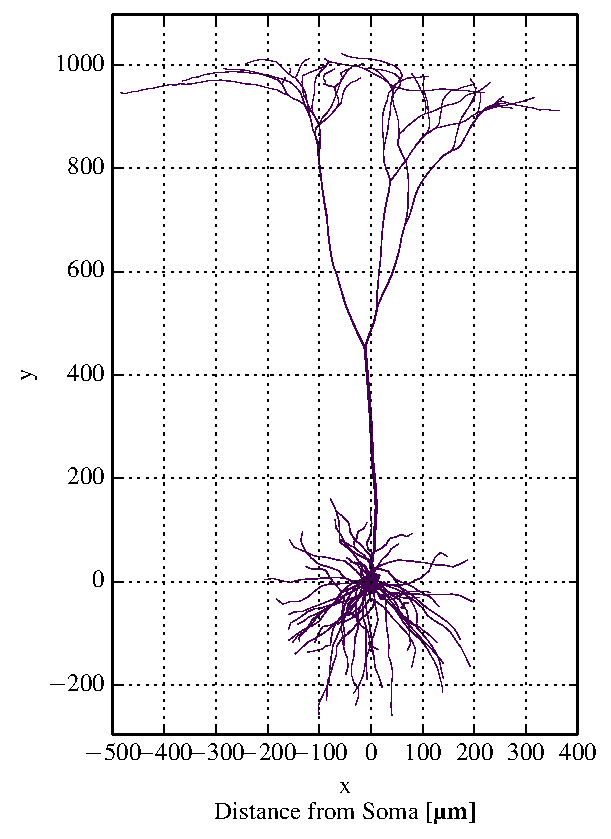
\includegraphics[width=\linewidth]{images/4_1/morph_xy_up.pdf}
        \vspace{-20pt}
        \caption{%
            Morphology of \textcite{mainen_influence_1996} cell. 
            The apical dendrites are located along the y-axis after rotation
            with PCA.}
        \label{fig:4_1_morph}
        \vspace{-10pt}
    \end{center}
\end{wrapfigure}
%
To verify that the simulation environment could be trusted 
some results from 
\textcite{pettersen_amplitude_2008} was replicated.
Spesifically the spike width and amplitude dependency in relation to 
the distance from soma was compared to current results. 

% {{{ Simulation%
\subsection{Simulation}
\textbf{Cell:}
The \textcite{mainen_influence_1996} morphology was used with a passive model, which is 
the same model used in \textcite{pettersen_amplitude_2008}. 
The cell was rotated using PCA (principal component analysis) on the compartment
positions.
This calculates three orthogonal vectors such that 
the positions of the compartments 
has the greatest variance along the first principal component, 
second highest along the second and third most along the third.
The first principal component was made paralell to the y-axis which
puts the apical dendrites along this axis
(\cref{fig:4_1_morph}).
\\

% CS model from Dayan Abott can be found in chapter 6, see fig 6.1 
% in the book.
\begin{figure}[h]
    \begin{center}
        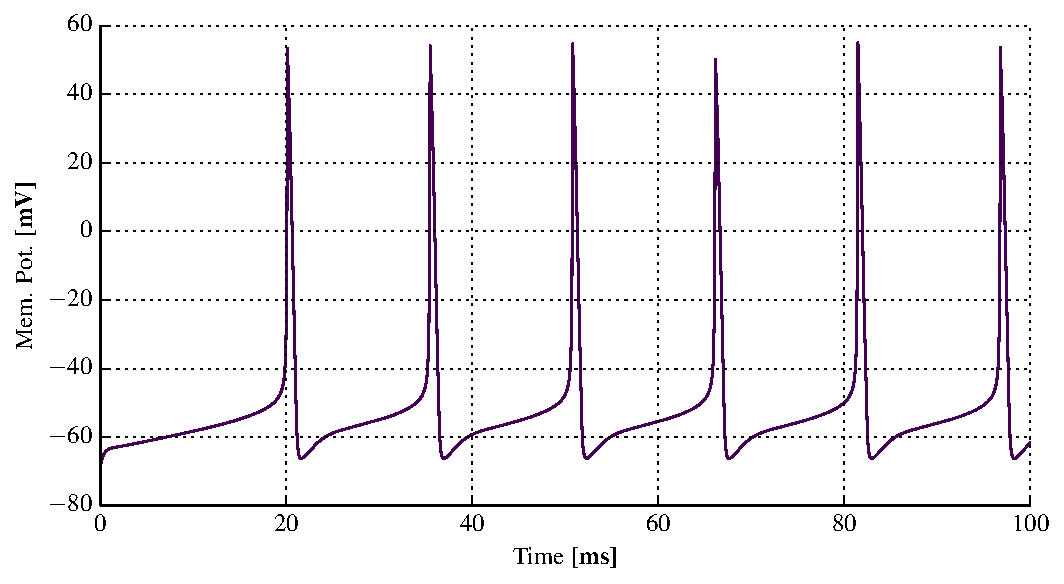
\includegraphics[width=1\textwidth]{images/4_1/cs_ap_original_signal.pdf}
        \caption{
            Simulation of the Connor-Stevens model using parameters from 
            \textcite{dayan_theoretical_2001}. A similar graph is shown in 
            fig. 6.1 (B) in their book.}
        \label{fig:4_1_cs_ap_signal}
    \end{center}
\end{figure}
\noindent
\textbf{Spike Generation:}
To recreate the action potential used in
\textcite{pettersen_amplitude_2008}
a spike was generated using the Connor-Stevens model 
(\textcite{connor_prediction_1971,connor_neural_1977})
using the same parameters as \textcite{dayan_theoretical_2001} and
\textcite{pettersen_amplitude_2008}\@. 
In \cref{fig:4_1_cs_ap_signal} the Connor-Stevens simulation is shown
where the second spike was used for further analysis. 
This spike had an amplitude of \SI{119.49}{\milli\volt} from baseline. 
The baseline was estimated to \SI{-53.26}{\milli\volt} and the
peak at \SI{53.26}{\milli\volt}. 
These values matches \textcite{dayan_theoretical_2001}\@, but not
the spike used in \textcite{pettersen_amplitude_2008} which had an amplitude of 
\SI{83}{\milli\volt} from baseline. 
\textcite{pettersen_amplitude_2008} does not go into further detail about
the creation of the action potential other than stating the action 
potential were similar to \textcite{dayan_theoretical_2001}\@.
The difference might be explained by the fact that action potentials
from pyramidal neurons often peaks at \SI{20}{\milli\volt},
and that this was achived by scaling the original signal from the
Connor-Stevens model.
To compensate for the difference the action potental used in further 
simulations were 
scaled to \SI{83}{\milli\volt} (\cref{fig:4_1_cs_ap_scaled}).

The input current was set to 
\SI{12.6}{\micro\ampere\per\centi\metre\squared}. 
and was very carefully adjusted to make the magnitude spectrum 
(\cref{fig:4_1_fourier})
similar to 
\textcite{pettersen_amplitude_2008}\@ figure 3.
Without adjustment the magnitude spectrum tended to have
a different inital value, from $6$ to \SI{8}{\milli\volt}, and
was not as smooth.
\\

\begin{figure}[h]
    \begin{center}
        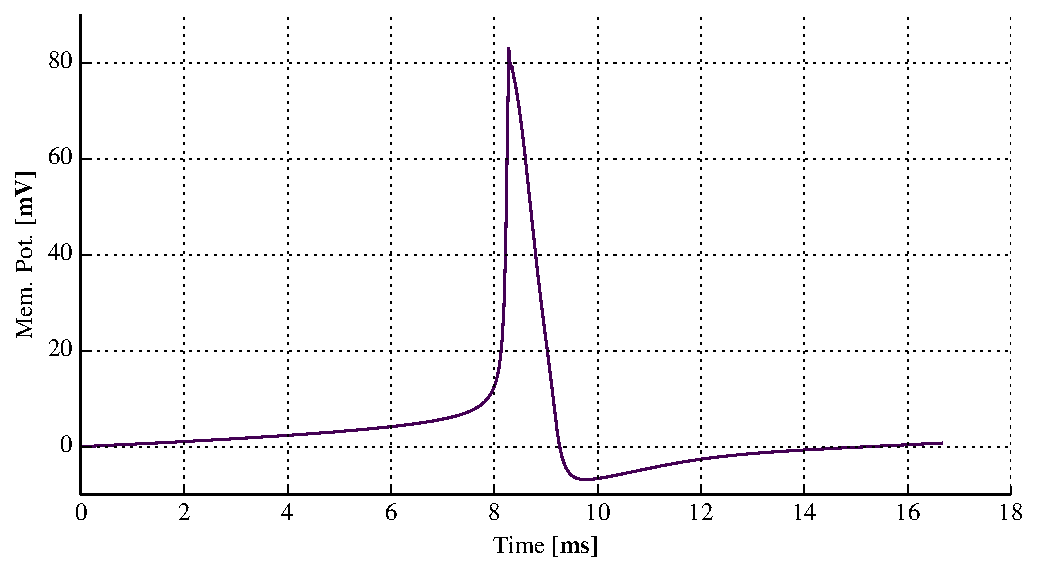
\includegraphics[width=1\textwidth]{images/4_1/cs_ap_scaled.pdf}
        \caption{
            The second spike in \cref{fig:4_1_cs_ap_signal} scaled to 
            \SI{83}{\milli\volt} to match the action potential used in 
            \textcite{pettersen_amplitude_2008}.
            }
        \label{fig:4_1_cs_ap_scaled}
    \end{center}
\end{figure}

\noindent
\textbf{Parameters:}
Parameters for the Neuron simulation were the same as 
\textcite{pettersen_amplitude_2008} and the aforementioned 
action potential was 
used as a boundary
condition in soma.
This was accomplished by 
setting the membrane potential equal to the 
action potential in all
soma sections using the 
{\verb .play }
vector function in Neuron.
This "excites" the neuron even though there are no
ion channels in the model.

Membrane resistance 
$R_m = \SI{30}{\kilo\ohm\per\centi\metre\squared}$, 
membrane capacitance 
$C_m=\SI{1}{\micro\farad\per\centi\metre\squared}$, 
axial resistance 
$R_a = \SI{150}{\ohm\per\centi\metre\squared}$, 
time resolution 
$dt = \SI[exponent-base=2]{e-5}{\milli\second}$. 
The reversal potential was set to zero. 
\\

\begin{wrapfigure}[19]{r}{.5\textwidth}
    \vspace{-20pt}
    \begin{center}
        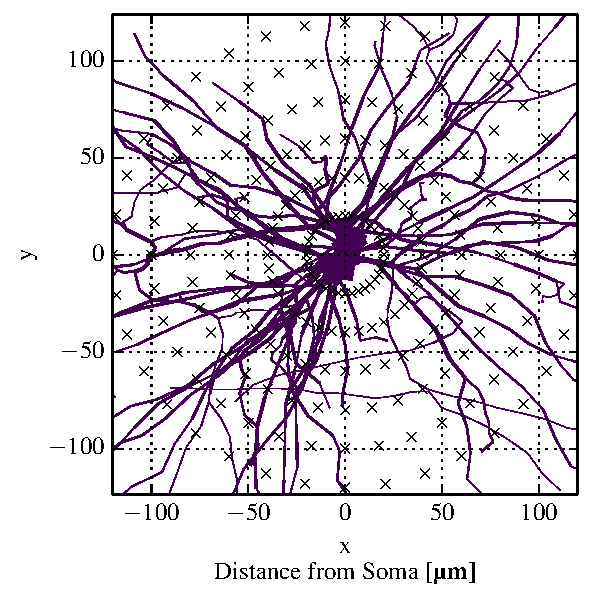
\includegraphics[width=\linewidth]{images/4_1/disc_morph_elec_xz.pdf}
        \vspace{-20pt}
        \caption{%
            Electrode positions placed in a plane around soma perpendicular to
            the axis along the apical dendrites.
            }
        \label{fig:4_1_electrode_pos}
        \vspace{-10pt}
    \end{center}
\end{wrapfigure}
\noindent
\textbf{Electrode Positions:}
Recording sites were placed in the xz-plane at 11 linearly spaced 
positions along 36 lines with equal 
angular spacing (\cref{fig:4_1_electrode_pos}).
\textcite{pettersen_amplitude_2008} states the recording positions
were in the plane perpendicular to the apical dendrites, this is 
ensured by the rotation done with PCA and putting the electrodes in
the xz-plane.
\\


\noindent
\textbf{Spike Width \& Amplitude:}
A baseline was set as the value at the start of the signal. 
Amplitude was calculated as the difference between the maximum value and the
baseline.
The spike width was calculated at as the width at half maximum value. 

At 
$dt = \SI[exponent-base=2]{e-5}{\milli\second}$,
the spike width from the Connor-Steven model was 
\SI{0.5625}{\milli\volt}.
This is similar to the reported spike width from
\textcite{pettersen_amplitude_2008} which was
was \SI{0.55}{\milli\second}.
Because the $dt$ used in their simulations was
$dt = \SI[exponent-base=2]{e-5}{\milli\second} = \SI{0.03125}{\milli\second}$,
their resulting spike width 
must have been rounded to
the nearest \SI{0.05}{\milli\second}.

% }}}  %
% {{{ Results %
\subsection{Results}
The action potental that was used in \textcite{pettersen_amplitude_2008} 
is similar to the one used here.  The amplitude of the fourier transform is displayed in
\cref{fig:4_1_fourier}, which is in close resemblance to the action potential
in fig. $3$ in the paper. 

\begin{figure}[thp]
    \centering
    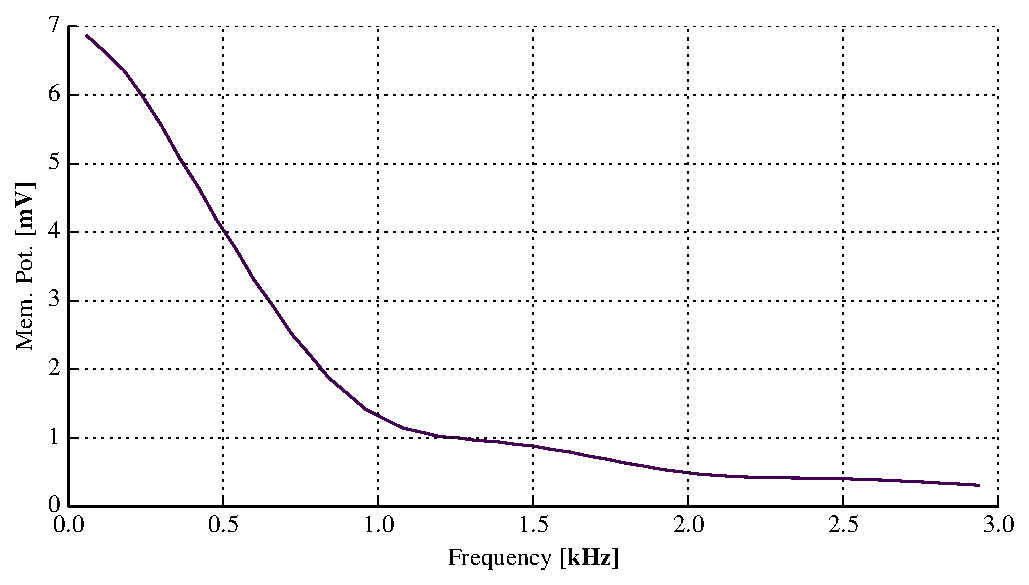
\includegraphics[width=\textwidth]{images/4_1/cs_ap_fourier.pdf}
    \caption{Magnitude specter of simulated somatic membrane potential.}
    \label{fig:4_1_fourier}
\end{figure}

The spike width increases with the distance from soma as seen in 
\cref{fig:4_1_spike_width}. 
These results are 
lower than the widths reported in \textcite{pettersen_amplitude_2008}.

Sudden changes in spike width was experienced with increased distance from
soma. Above $200\mu V$ the
most of the spikes shapes are not well defined. 
This was also reported in \textcite{pettersen_amplitude_2008}\@.

\Cref{fig:4_1_spike_amp} shows the spike amplitude with logarithmic axes.  
The exact results from 
\textcite{pettersen_amplitude_2008}
are not available but 
the approximate value can be seen from their plots and
the exponential decay
$1 / r^n$
was reported
as  $n \sim 2$ at \SI{20}{\micro\metre} and 
$n \sim 2.5$ at \SI{120}{\micro\metre}.
Current results are not identical to those findings
and have an exponent 
of $n = 2$ at \SI{20}{\micro\metre}
and $n = 2.8$ at \SI{120}{\micro\metre}.
The value of the amplitude was about
\SI{350}{\micro\volt} in 
\textcite{pettersen_amplitude_2008}, 
but the current model only gives an amplitude of 
\SI{120}{\micro\volt} 
at 
\SI{20}{\micro\metre}.
How can I explain this descrepancy?

\begin{figure}[thp]
\centering
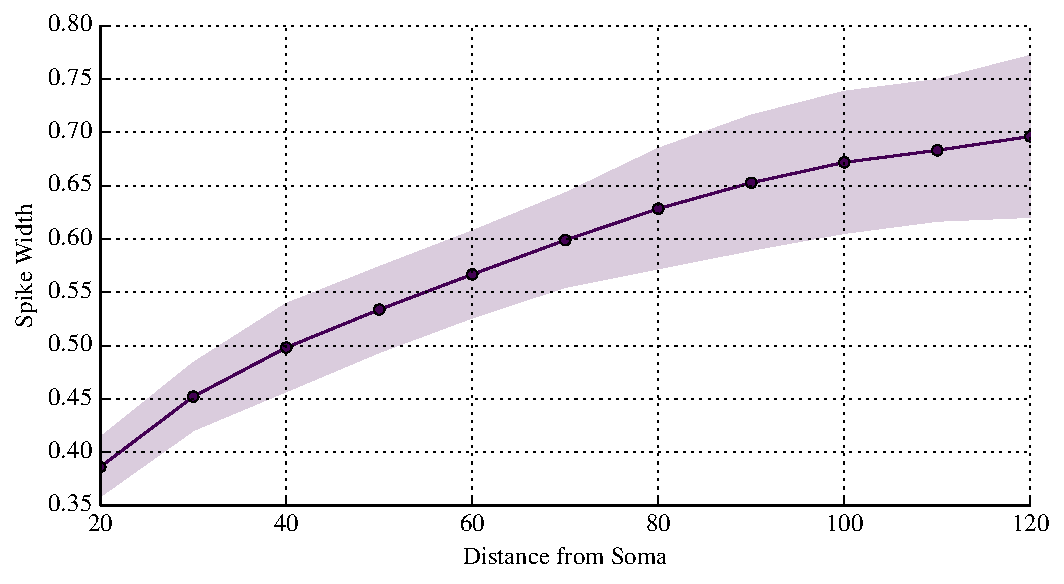
\includegraphics[width=\textwidth]{images/4_1/disc_spike_width_II.pdf}
\caption{Spike width over distance. Mean +/- 1 std.}
\label{fig:4_1_spike_width}
\end{figure}

\begin{figure}[thp]
    \centering
    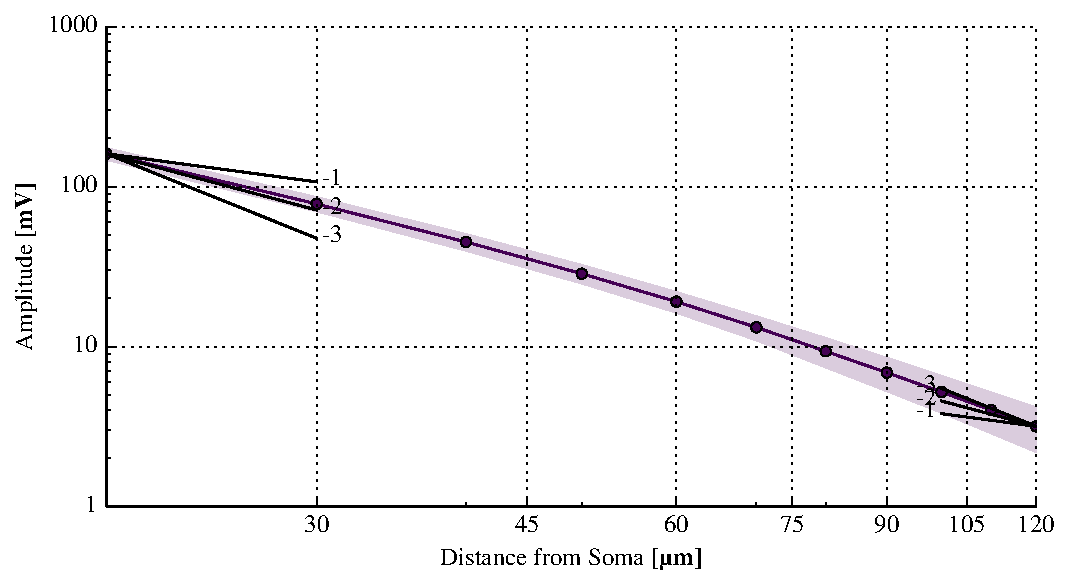
\includegraphics[width=\textwidth]{images/4_1/disc_spike_amps_I_log.pdf}
    \caption{Spike amplitude over distance. Mean +/- 1 std. The power law
    decays $1/r$, $1/r^2$ and $1/r^3$ are shown at the leftmost and rightmost
    data points.}
    \label{fig:4_1_spike_amp}
\end{figure}
% }}}  %
% {{{ Discussion%
% \subsection{Discussion}

% }}}  %
%}}} end of Pettersen and Einvoll
% {{{ Optimal Spike Width%
\newpage
\section{Optimal Width Definition}
\begin{wrapfigure}[17]{r}{.5\textwidth}
    \vspace{-20pt}
    \begin{center}
        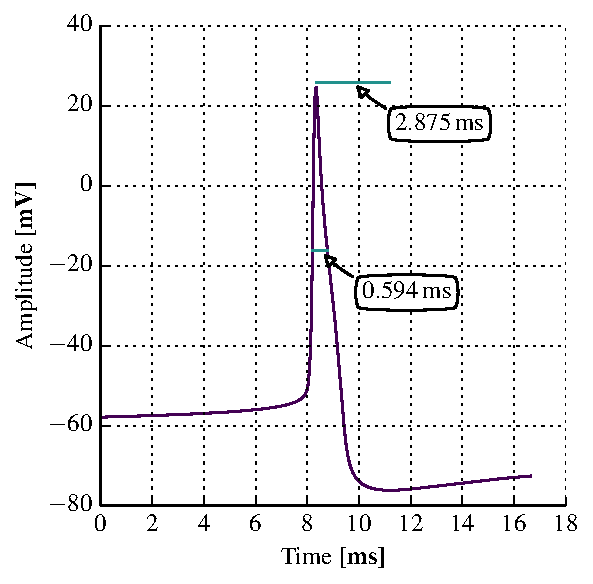
\includegraphics[width=\linewidth]{images/4_2/widthdef_soma_mem_small.pdf}
        \vspace{-20pt}
        \caption{%
            Width types.
            }
        \label{fig:4_2_width_def}
        \vspace{-10pt}
    \end{center}
\end{wrapfigure}
Many different definitions of spike width has been used to differentiate neurons,
and some investigation hase gone into which definitions are best suited
for classification. 
Notebly Bartho 2004 concluded that of all the spike features investigated, 
the spike durtion most reliably gave the best seperation between pyramidal and
interneurons
in the somatosensory cortex and prefrontal cortex for both the anethesiased
and the drug-free animals. 
Moreover they suggested that the peak-to-peak width definition
of the unfiltered trace reliably gave the better bimodal distributions

% This section covers an analysis of two different commonly used spike definitions
% that have been used to classify interneurons and pyramidal neurons.
The two width definitions analyzed are
the peak-to-peak spike definition and 
width at half amplitude from baseline,
respectively referred to as Type I and Type II
(\cref{fig:4_2_width_def}).
\newline

% Make plot of width over width. 

\noindent
\textbf{Models:}
To investigate which of the two 
width definitions is more optimal for differentiating
interneurons from pyramidal neurons,
three classes of the most abundant neurons were selected 
from the blue brain models.
Two classes of interneurons and one class of pyramidal neurons. 
There were two classes of pyramidal models available but as the
one class had identical dendrites it was not analyzed.
The number of inhibitory neuron classes were much greater,
the two classes were selected by being the most abundant 
inhibitory neurons in the L5 area.
In addition to these classes, one addition group
was analyzed named "All Inter." 
which included all available interneuron
models in L5.
In this group many of the classes represent only
a very small portion of the number of neurons in L5. 
The findings from 
\textcite{markram_reconstruction_2015} 
suggest
that overall the ratio between excitatory
and inhibitory neurons is around $87\% \pm 1\%$. 
Of these, $50\%$ were classified as 
baskets cells (LBC and NBC).
The interneurons from L5 were seperated into 
9 m-types (morphological) and 10 e-types (electrophysiological)
which gave a total number
of 48 uniquie models.
As such some small classes of 
interneurons are overrepresented in the grouped called "All Inter.".

The classes of neurons were Thick Thufted Pyramidal Cell with
an early bifurcating apical thuft (TTPC2), Large Basket Cell (LBC) and
Nest Basket Cell (NBC).
Each of the three class had 5 seperate models where each model
had different m-type but identical e-type.
The e-type of TTPC2 class was continuous adapting (cAD), 
LBC was delayed stuttering (dSTUT) 
and NBC was continuous non-accommodating (cNAC) 
(\textcite[463]{markram_reconstruction_2015}).
Simulations were ran using using the
SphereRand (\cref{sec:simulation_list}) simulation .
\newline

\noindent
\textbf{Seperation:}
A good definition is recoqnized by having a better
seperation between inhibitory
and excitatory neurons.
The results of the simulations can be seen in 
\cref{fig:4_2_width}.
For both deifinitions the spike width of interneurons are smaller
than the width of pyramidal neurons. 
These findings are in line with previously established research.
With the Type I definition the seperation between the two classes 
are greater in both absolute and relative value for all distances from soma.
The seperation between the mean of pyramidal and interneurons 
for Type I were 
\SI{0.40}{\milli\second} at \SI{30}{\micro\metre}
and 
\SI{0.60}{\milli\second} at \SI{100}{\micro\metre}.
For Type II the seperation was 
\SI{0.15}{\milli\second} at \SI{30}{\micro\metre}
and 
\SI{0.35}{\milli\second} at \SI{100}{\micro\metre}.
These results suggests that using a type I deifinition of the spike width
increases the chance of correctly classifying the neuron class.
\newline


\begin{figure}[h]
    \begin{center}
        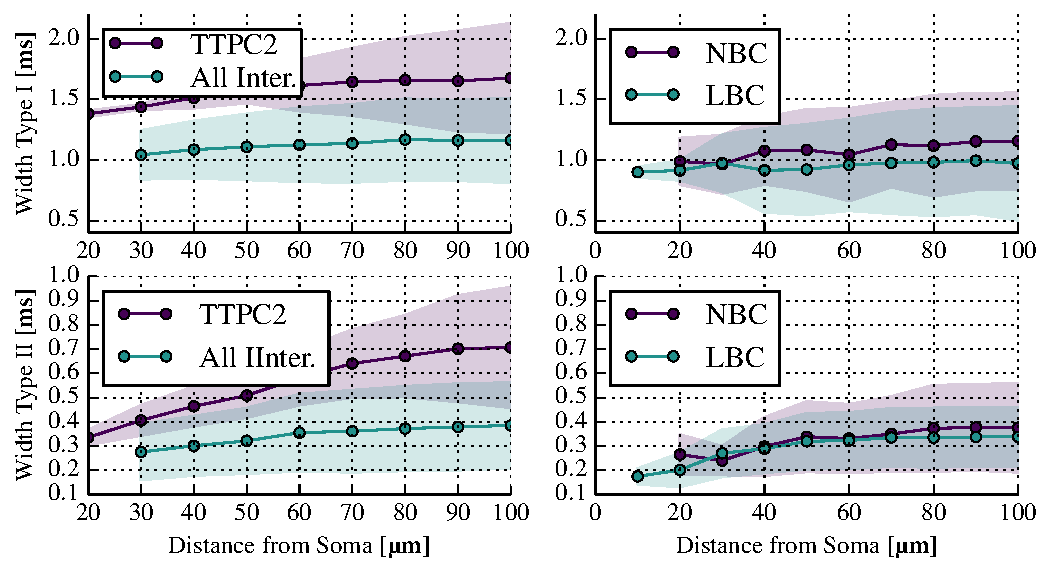
\includegraphics[width=1\textwidth]{images/4_2/TTPC2_NBC_LBC_IN_widths.pdf}
        \caption{
            Nothing.
        }
        \label{fig:4_2_width}
    \end{center}
\end{figure}

\noindent
\textbf{Variance:}
To evaluate the precision of the two width definitions
it is not very useful to compare the raw variance because 
the mean values are different.
An example is the $\sigma$ at 
\SI{50}{\micro\metre}
for the group "All Inter" from \cref{fig:4_2_width}.
For Type I 
$\sigma = \SI{0.25}{\milli\second}$ 
and 
$\mu = \SI{1.1}{\milli\second}$, 
while for Type II 
$\sigma = \SI{0.15}{\milli\second}$ 
and 
$\mu = \SI{0.3}{\milli\second}$. 
The variance is lower for Type II but is also
almost $50\%$ of the mean value. 
The variance from Type I is higher, but is only about 
$25\%$ of the mean value, 
which makes Type I more accurate than Type II.

The coefficient of variation, $c_v$,
is the relative variance compared to the mean.
\begin{align}
    c_v = \frac{\sigma}{\mu}
\end{align}
Because the variance is of similar magnitude for both width definitions, 
the overall greater mean of the Type I definition results in a
lesser $c_v$ at all distances, for all groups except LBC
(\cref{fig:4_2_width_snr}).
To minimalize errors when classifing neurons based on width 
it is best to minize the overlap between the two definitions.
Because the seperation is higher and $c_v$ is lower with Type I,
this definition is better suited for classification.

\begin{figure}[h]
    \begin{center}
        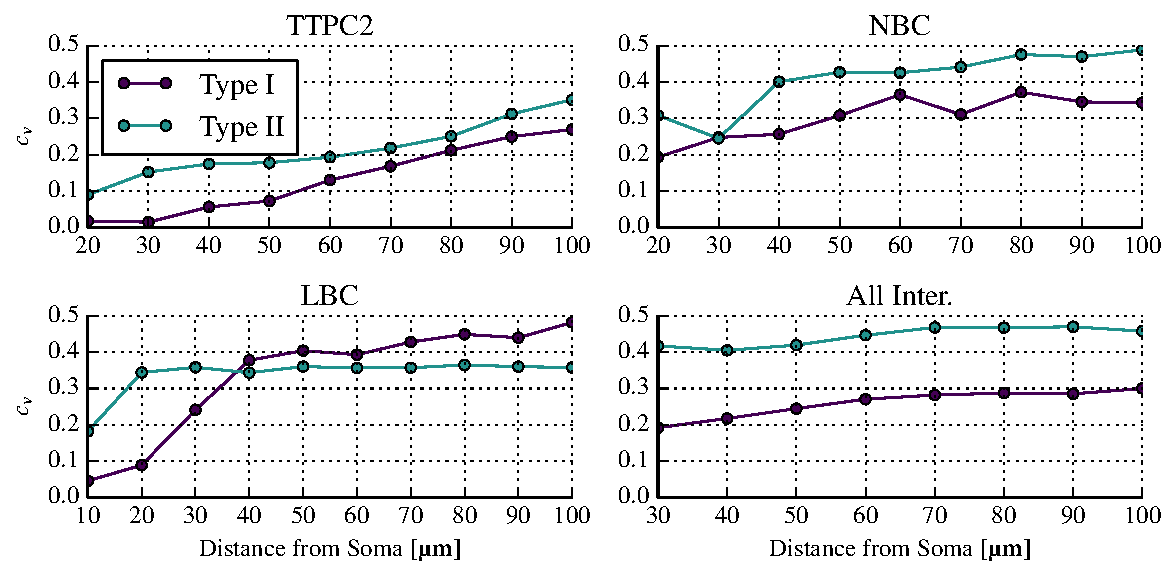
\includegraphics[width=1\textwidth]{images/4_2/TTPC2_NBC_LBC_IN_snr.pdf}
        \caption{
            Nothing.
        }
        \label{fig:4_2_width_snr}
    \end{center}
\end{figure}

The distance from the soma is usually unknown in most extracellular 
recording experiments so measurements from random positions around 
withing a distance of XX of the soma has been collected. 



\noindent
% }}}  %
% {{{  Optimal Amplitude Definition%
% \section{Optimal Amplitude Definition}
% \begin{figure}[h]
%     \begin{center}
%         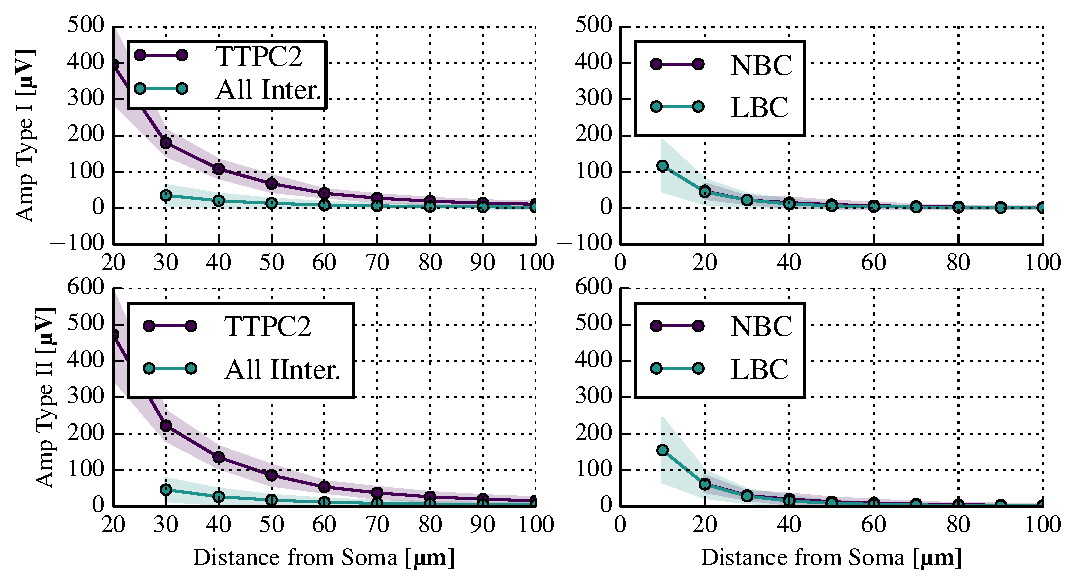
\includegraphics[width=1\textwidth]{images/4_2/TTPC2_NBC_LBC_IN_amps.pdf}
%         \caption{
%             Nothing.
%         }
%         \label{fig:4_2_amp}
%     \end{center}
% \end{figure}
% The two amplitude definitions investigated are
% the amplitude from baseline (Type I) and 
% the peak-to-peak amplitude definition (Type II).
% The simulations were ran using the same neurons and simulations
% as the previous section.

% \Cref{fig:4_2_amp} shows the 

% }}}  %
% {{{ Classifying Neurons%
\section{Classifying Inter and Pyramidal Neurons}


Classification using computer methods is a field in much development where new
methods are emerging rapidly. 
Classification of neurons based on this data could probably be done better 
using computer methods, but still it is useful to have a metric 
to measure similarity between models. 
% To measure the similarity between two models the histograms of the
% spike width and spike amplitude has been compared. 
The jaccard coefficient is a measurement that can be used to compute
the overlap between two histograms and has been used here to compare the 
models against each other. 
Picture ** shows a comparison between each model using the jaccard coefficient
of the histograms. 
% Blue brain reconstruced neurons and indentified 55 types of 
% morphological structures. 

% Excitatory neurons represented above $87\%$ of all neurons in L5.

% 50 \% of all inhibitory interneurons are baskets cells (LBC and NBC),
% these types have been simulated.


% All models from blue brain from L5 was ran using the SphereRand simulation and were
% divided between interneurons and pyramidal neurons. 


% }}} 
% Comparing results {{{ %
\section{Comparing Results}
Bartho 2004, spike widths  = 0.43 +- 0.27 ms than that of the
putative pyramidal cells 0.86 +- 0.17 ms.

% }}} Comparing results %
%}}} end of Results
%{{{ Discussion
\chapter{Discussion}

% TODO: Fill
Spike Width and Spike Amplitude:
It has been seen that of the spike width definitions investigated here, 
one type of spike width definition is overall
better suited to classify this set of neurons. 
This has also been seen in the literature. 
A similar investigation was done using the spike amplitude and of the
definitions investigated here the peak-to-peak amplitude gave the best
seperation between interneuron and pyramidal neurons. 

Classification:
It has been previously shown that using only spike width as 
a way to classify neurons is not the best. 
Several papers have stated that other methods can be used to give 
a clearer distinction, such as considering the interspike interval. 
Also one group looked at the spike width from axons which gave a short 
durtion. 

Using a simple measure of the similarity between populations
neuron models it can be clearly stated that interneurons can be seperated
from pyramidal neurons. 
Excitatory interneurons cannot be clearly distinguished from the rest of the
interneurons. 
Using machine learning algorithms it might be possible to divide these
into even small groups, how can I show this?
Neurons could probably be seperated into smaller groups based on
spike width and spike amplitude. 

% TODO: Fill
LFPyUtil: 
LFPyUtil is a useful tool that can be used to easily gather
new data when new models arrive. 
As long as a model has the mechanics defined with NEURON and has
a morphology the same simulations and data as seen here can be ran 
and extraced.

% TODO: Fill
The models did now show the expected variance with firing frequency. 
% Article anastassiou is consistent with Nature review, spike shape increases with 
% frequency. 
% This is not the case the models from Blue Brain.

% TODO: Fill
Comparisons with other data:
several articles was investigated to compare current data with.
There is a large variance in the literature of spike widths and amplitude. 
All in all the data fall within the variance of the investigated articles. 
The number range between this and that.


Sources of variation:

% Results are based on spike width and amplitude.
% The basis for all spike shapes are the types and concentrations of
% ion channels.
% This is the central factor that decides if the neuron has short or long action potentials.
% A number things has been observed that can change spike spike width.
% Factors that change action potentials width:
% * Firing frequency.
% * Input current. Higher current gives higher frequency.
% * Number of previous spikes.
% * Bursting behavior.
% * Backproagating action potentials.

% % What are the results, what do you want to show.
% % The grand wish, have a catalogue of all spikes in the brain.
% When plotting spike amplitude over spike width will neurons look different.

% Results: Spike width alone is often used for classifying neurons.
% They often have a bimodal distribution. 
% This is the first time many simulations have been done of the extracellular
% potential.
% Previous research have only used a few models.
% With LFPy and LFPyUtil it will be easy to adapt new models to calculate extracellular potential.

% The spike widths does not show dependency on the firing frequency or spike number.
% Some neurons show this feature and this should do it too.

% Results:
% * Which width and amp definition is most suitable for differention.
% * Classify neurons based on spike width and amplitude.
%     * Compare to other data. 
%     Hard to varify model,
%     values from experiments are vary a lot. 
%     Models were based on result from their recordings. 
%     Cannot see adaption with frequency of any kind.
%     * Is experimental distribution shape similar to mine, if so
%     that is a good result.
% * Development of LFPyUtil. Future neuron models can be adapted for 
% extracellular simulations if they include
% a morphology.

%}}} end of Discussion
% % Appendix {{{ %
\begin{appendices}
\chapter{Appendix}
% \begin{listing}[H]
%     \caption{load\_model.py - A function to load a Cell object.}
% \begin{mdframed}
    \inputminted[
        breaklines=true,
        frame=lines,
        baselinestretch=0.4,
        fontsize=\footnotesize,
        bgcolor=LightGray,
        linenos
    ]{python}{examples/load_model.py}
    % \label{code:load_model}
% \end{listing}
% \end{mdframed}
% }}} Appendix %
\end{appendices}
%{{{ Bibliography
\nocite{*}
\printbibliography[heading=bibintoc]
% }}}
\end{document}
